\section{Lineares Hashing 2}

Gegeben ist die unten skizzierte lineare Hashtabelle mit $q = 4$ Buckets, die jeweils eine Größe $b = 1$ besitzen. Es wurde bisher 1 vorgegebener Schlüssel in die Tabelle eingefügt und es wurden noch keine Verdopplungen ausgeführt. Positionszeiger $p = 0$. Die Folge von Hashfunktionen sei $h_{j}(k) = k \bmod(2^{j} \cdot q), \; j = 0,1, \ldots$ .

\begin{minipage}{5cm}
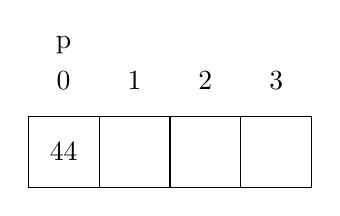
\begin{tikzpicture}
	\draw[step=0.9cm] (0, 0) grid +(3.6, 0.9);
	\node at (0.45, 0.45) {44};
	\node at (0.45, 1.8) {p};
	\node at (0.45, 1.35) {0};
	\node at (1.35, 1.35) {1};
	\node at (2.25, 1.35) {2};
	\node at (3.15, 1.35) {3};
\end{tikzpicture}
\end{minipage}\hfill
\begin{minipage}{0.65\textwidth}
Belegungsfaktor:
\[\beta = \frac{N}{ (q \cdot 2^{L} + p) \cdot b} = \frac{1}{(4 \cdot 2^{0} + 0) \cdot 1} = 0,25\]
\end{minipage}

Fügen Sie die folgenden Schlüssel in der angegebenen Reihenfolge in die Tabelle ein. Verwenden Sie dabei kontrolliertes Splitting mit Schwellenwert $\alpha = 0,7$. \\
6, 15, 57, 2, 8

\begin{note}
Folgende Hashfunktionen kommen zum Einsatz:
\begin{itemize}
	\item $h_{0}(k) = k \bmod (2^0 \cdot 4) = k \bmod 4$
	\item $h_{1}(k) = k \bmod (2^1 \cdot 4) = k \bmod 8$
	\item $h_{2}(k) = k \bmod (2^2 \cdot 4) = k \bmod 16$
\end{itemize}

%1
\begin{minipage}{0.4\textwidth}
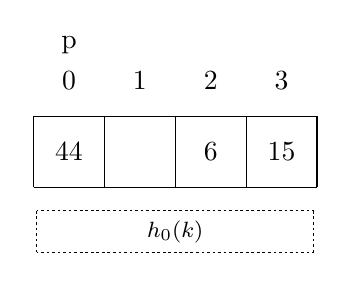
\begin{tikzpicture}
	%template
	\draw[step=0.9cm] (0, 0) grid +(3.6, 0.9);
	\node at (0.45, 0.45) {44};
	\node at (2.25, 0.45) {6};
	\node at (3.15, 0.45) {15};
	\node at (0.45, 1.8) {p};
	\node at (0.45, 1.35) {0};
	\node at (1.35, 1.35) {1};
	\node at (2.25, 1.35) {2};
	\node at (3.15, 1.35) {3};
	%hash functions
	\node at (1.8, -0.55) {\dashbox{1}(100,15){\footnotesize $h_0(k)$}};
\end{tikzpicture}
\end{minipage}
\begin{minipage}{0.55\textwidth}
Einfügen der Schlüssel 6 und 15 lässt $\beta > \alpha$ werden: \\
\[\beta = \frac{N}{ (q \cdot 2^{L} + p) \cdot b} = \frac{3}{(4 \cdot 2^{0} + 0) \cdot 1} = \textcolor{red}{0,75}\]
\end{minipage}

%2
\begin{minipage}{0.4\textwidth}
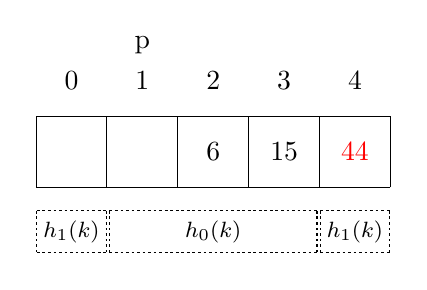
\begin{tikzpicture}
	%template
	\draw[step=0.9cm] (0, 0) grid +(4.5, 0.9);
	\node at (2.25, 0.45) {6};
	\node at (3.15, 0.45) {15};
	\node at (4.05, 0.45) {\textcolor{red}{44}};
	\node at (1.35, 1.8) {p};
	\node at (0.45, 1.35) {0};
	\node at (1.35, 1.35) {1};
	\node at (2.25, 1.35) {2};
	\node at (3.15, 1.35) {3};
	\node at (4.05, 1.35) {4};
	%hash
	\node at (2.25, -0.55) {\dashbox{1}(75,15){\footnotesize $h_0(k)$}};
	\node at (4.05, -0.55) {\dashbox{1}(25,15){\footnotesize $h_1(k)$}};
	\node at (0.45, -0.55) {\dashbox{1}(25,15){\footnotesize $h_1(k)$}};
\end{tikzpicture}
\end{minipage}
\begin{minipage}{0.55\textwidth}
Splitt von Bucket 0, es werden jetzt $h_0(k)$ und $h_1(k)$ angewendet. \\
\[\beta = \frac{N}{ (q \cdot 2^{L} + p) \cdot b} = \frac{3}{(4 \cdot 2^{0} + 1) \cdot 1} = {0,6}\]
\end{minipage}

%3
\begin{minipage}{0.4\textwidth}
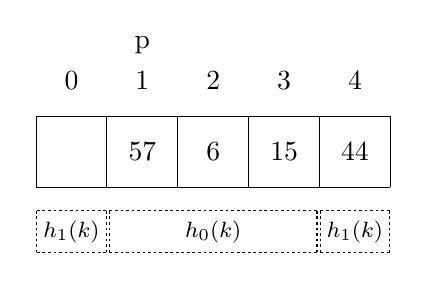
\begin{tikzpicture}
	%template
	\draw[step=0.9cm] (0, 0) grid +(4.5, 0.9);
	\node at (1.35, 0.45) {57};
	\node at (2.25, 0.45) {6};
	\node at (3.15, 0.45) {15};
	\node at (4.05, 0.45) {44};
	\node at (1.35, 1.8) {p};
	\node at (0.45, 1.35) {0};
	\node at (1.35, 1.35) {1};
	\node at (2.25, 1.35) {2};
	\node at (3.15, 1.35) {3};
	\node at (4.05, 1.35) {4};
	%hash
	\node at (2.25, -0.55) {\dashbox{1}(75,15){\footnotesize $h_0(k)$}};
	\node at (4.05, -0.55) {\dashbox{1}(25,15){\footnotesize $h_1(k)$}};
	\node at (0.45, -0.55) {\dashbox{1}(25,15){\footnotesize $h_1(k)$}};
\end{tikzpicture}
\end{minipage}
\begin{minipage}{0.55\textwidth}
Einfügen des Schlüssels 57 lässt $\beta > \alpha$ werden: \\
\[\beta = \frac{N}{ (q \cdot 2^{L} + p) \cdot b} = \frac{4}{(4 \cdot 2^{0} + 1) \cdot 1} = \textcolor{red}{0,8}\]
\end{minipage}

%4
\begin{minipage}{0.4\textwidth}
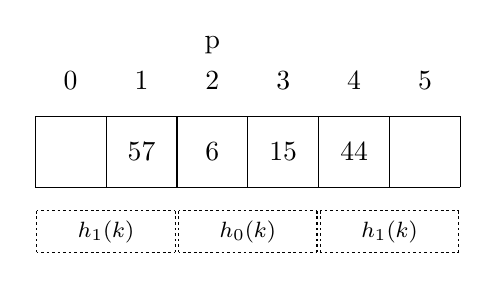
\begin{tikzpicture}
	%template
	\draw[step=0.9cm] (0, 0) grid +(5.4, 0.9);
	\node at (1.35, 0.45) {57};
	\node at (2.25, 0.45) {6};
	\node at (3.15, 0.45) {15};
	\node at (4.05, 0.45) {44};
	\node at (2.25, 1.8) {p};
	\node at (0.45, 1.35) {0};
	\node at (1.35, 1.35) {1};
	\node at (2.25, 1.35) {2};
	\node at (3.15, 1.35) {3};
	\node at (4.05, 1.35) {4};
	\node at (4.95, 1.35) {5};
	%hash
	\node at (2.7, -0.55) {\dashbox{1}(50,15){\footnotesize $h_0(k)$}};
	\node at (4.5, -0.55) {\dashbox{1}(50,15){\footnotesize $h_1(k)$}};
	\node at (0.9, -0.55) {\dashbox{1}(50,15){\footnotesize $h_1(k)$}};
\end{tikzpicture}
\end{minipage}
\begin{minipage}{0.55\textwidth}
Splitt von Bucket 1 \\
\[\beta = \frac{N}{ (q \cdot 2^{L} + p) \cdot b} = \frac{4}{(4 \cdot 2^{0} + 2) \cdot 1} = {0,67}\]
\end{minipage}

%5
\begin{minipage}{0.4\textwidth}
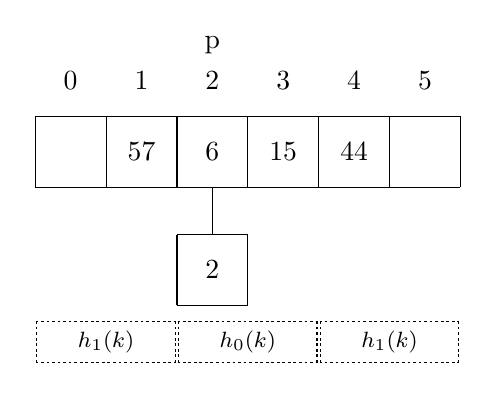
\begin{tikzpicture}
	%template
	\draw[step=0.9cm] (0, 0) grid +(5.4, 0.9);
	\draw (1.8, -1.5) -- (1.8, -0.6);
	\draw (2.25, 0) -- (2.25, -0.6);
	\draw (2.7, -1.5) -- (2.7, -0.6);
	\draw (1.8, -1.5) -- (2.7, -1.5);
	\draw (1.8, -0.6) -- (2.7, -0.6);
	\node at (1.35, 0.45) {57};
	\node at (2.25, 0.45) {6};
	\node at (3.15, 0.45) {15};
	\node at (4.05, 0.45) {44};
	\node at (2.25, -1.05) {2};
	\node at (2.25, 1.8) {p};
	\node at (0.45, 1.35) {0};
	\node at (1.35, 1.35) {1};
	\node at (2.25, 1.35) {2};
	\node at (3.15, 1.35) {3};
	\node at (4.05, 1.35) {4};
	\node at (4.95, 1.35) {5};
	%hash
	\node at (2.7, -1.95) {\dashbox{1}(50,15){\footnotesize $h_0(k)$}};
	\node at (4.5, -1.95) {\dashbox{1}(50,15){\footnotesize $h_1(k)$}};
	\node at (0.9, -1.95) {\dashbox{1}(50,15){\footnotesize $h_1(k)$}};
\end{tikzpicture}
\end{minipage}
\begin{minipage}{0.55\textwidth}
Einfügen des Schlüssels 2 lässt $\beta > \alpha$ werden: \\
\[\beta = \frac{N}{ (q \cdot 2^{L} + p) \cdot b} = \frac{5}{(4 \cdot 2^{0} + 2) \cdot 1} = \textcolor{red}{0,83}\]
\end{minipage}


%6
Splitt von Bucket 2. Dennoch weiterhin $\beta > \alpha$:\\

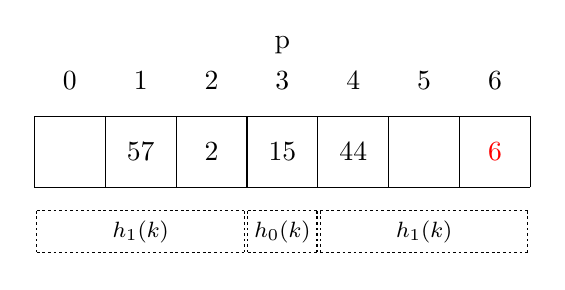
\begin{tikzpicture}
	%template
	\draw[step=0.9cm] (0, 0) grid +(6.3, 0.9);
	\node at (1.35, 0.45) {57};
	\node at (2.25, 0.45) {2};
	\node at (3.15, 0.45) {15};
	\node at (4.05, 0.45) {44};
	\node at (5.85, 0.45) {\textcolor{red}{6}};
	\node at (3.15, 1.8) {p};
	\node at (0.45, 1.35) {0};
	\node at (1.35, 1.35) {1};
	\node at (2.25, 1.35) {2};
	\node at (3.15, 1.35) {3};
	\node at (4.05, 1.35) {4};
	\node at (4.95, 1.35) {5};
	\node at (5.85, 1.35) {6};
	%hash
	\node at (3.15, -0.55) {\dashbox{1}(25,15){\footnotesize $h_0(k)$}};
	\node at (4.95, -0.55) {\dashbox{1}(75,15){\footnotesize $h_1(k)$}};
	\node at (1.35, -0.55) {\dashbox{1}(75,15){\footnotesize $h_1(k)$}};
\end{tikzpicture}

\[\beta = \frac{N}{ (q \cdot 2^{L} + p) \cdot b} = \frac{5}{(4 \cdot 2^{0} + 3) \cdot 1} = {0,71}\]

%7
Splitt von Bucket 3:

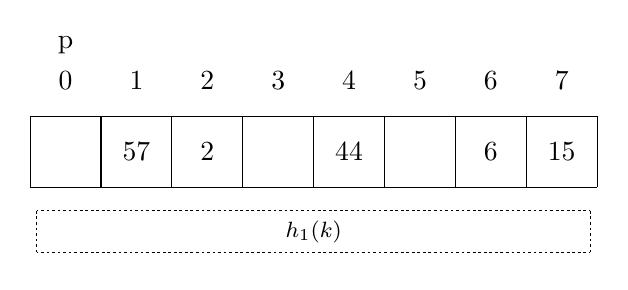
\begin{tikzpicture}
	%template
	\draw[step=0.9cm] (0, 0) grid +(7.2, 0.9);
	\node at (1.35, 0.45) {57};
	\node at (2.25, 0.45) {2};
	\node at (4.05, 0.45) {44};
	\node at (5.85, 0.45) {6};
	\node at (6.75, 0.45) {15};
	\node at (0.45, 1.8) {p};
	\node at (0.45, 1.35) {0};
	\node at (1.35, 1.35) {1};
	\node at (2.25, 1.35) {2};
	\node at (3.15, 1.35) {3};
	\node at (4.05, 1.35) {4};
	\node at (4.95, 1.35) {5};
	\node at (5.85, 1.35) {6};
	\node at (6.75, 1.35) {7};
	%hash
	\node at (3.60, -0.55) {\dashbox{1}(200,15){\footnotesize $h_1(k)$}};
\end{tikzpicture}

\[\beta = \frac{N}{ (q \cdot 2^{L} + p) \cdot b} = \frac{5}{(4 \cdot 2^{1} + 0) \cdot 1} = {0,625}\]

%8
Einfügen des Schlüssels 8 lässt $\beta > \alpha$ werden: \\

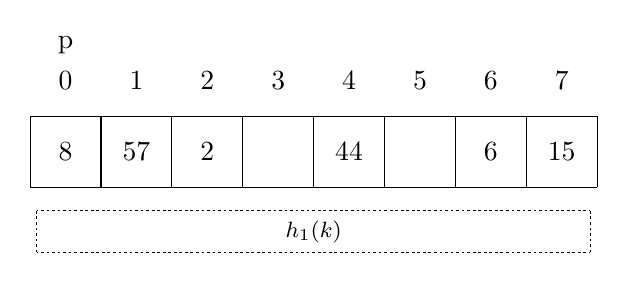
\begin{tikzpicture}
	%template
	\draw[step=0.9cm] (0, 0) grid +(7.2, 0.9);
	\node at (0.45, 0.45) {8};
	\node at (1.35, 0.45) {57};
	\node at (2.25, 0.45) {2};
	\node at (4.05, 0.45) {44};
	\node at (5.85, 0.45) {6};
	\node at (6.75, 0.45) {15};
	\node at (0.45, 1.8) {p};
	\node at (0.45, 1.35) {0};
	\node at (1.35, 1.35) {1};
	\node at (2.25, 1.35) {2};
	\node at (3.15, 1.35) {3};
	\node at (4.05, 1.35) {4};
	\node at (4.95, 1.35) {5};
	\node at (5.85, 1.35) {6};
	\node at (6.75, 1.35) {7};
	%hash
	\node at (3.60, -0.55) {\dashbox{1}(200,15){\footnotesize $h_1(k)$}};
\end{tikzpicture}

\[\beta = \frac{N}{ (q \cdot 2^{L} + p) \cdot b} = \frac{6}{(4 \cdot 2^{1} + 0) \cdot 1} = {0,75}\]

%9
Splitt von Bucket 0, $h_2(k)$ kommt hinzu:

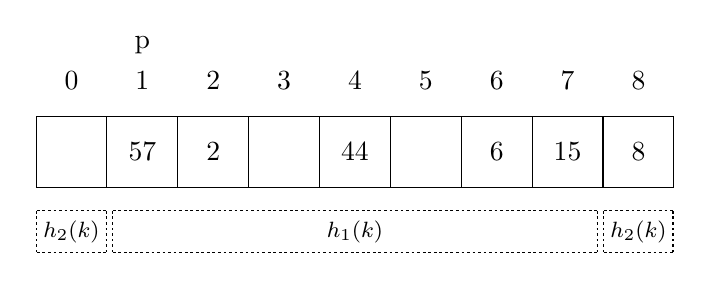
\begin{tikzpicture}
	%template
	\draw[step=0.9cm] (0, 0) grid +(8.1, 0.9);
	\node at (1.35, 0.45) {57};
	\node at (2.25, 0.45) {2};
	\node at (4.05, 0.45) {44};
	\node at (5.85, 0.45) {6};
	\node at (7.65, 0.45) {8};
	\node at (6.75, 0.45) {15};
	\node at (1.35, 1.8) {p};
	\node at (0.45, 1.35) {0};
	\node at (1.35, 1.35) {1};
	\node at (2.25, 1.35) {2};
	\node at (3.15, 1.35) {3};
	\node at (4.05, 1.35) {4};
	\node at (4.95, 1.35) {5};
	\node at (5.85, 1.35) {6};
	\node at (6.75, 1.35) {7};
	\node at (7.65, 1.35) {8};
	%hash
	\node at (4.05, -0.55) {\dashbox{1}(175,15){\footnotesize $h_1(k)$}};
	\node at (7.65, -0.55) {\dashbox{1}(25,15){\footnotesize $h_2(k)$}};
	\node at (0.45, -0.55) {\dashbox{1}(25,15){\footnotesize $h_2(k)$}};
\end{tikzpicture}

\[\beta = \frac{N}{ (q \cdot 2^{L} + p) \cdot b} = \frac{6}{(4 \cdot 2^{1} + 1) \cdot 1} = {0,67}\]

\end{note}
